\documentclass[11pt]{article}

\usepackage{fancyhdr}
\usepackage{cite}
\usepackage{amsmath}
%\usepackage{swmacros}
\usepackage{graphicx}
\usepackage{float}
\usepackage{color}


\usepackage[top=1in, bottom=1in, left=.5in, right=.5in]{geometry}
%\usepackage[font=small,labelfont=bf]{caption}

\setlength\parindent{0pt}
% Title.
% ------
\title{STAT 240 Final Project}
\author{Rebecca Barter, Andrew Do and Kellie Ottoboni}



\begin{document}

\maketitle

 \section{Introduction}
Over the last two decades developing countries have seen an increase in the number of new primary school entrants, driven in part by the elimination of school fees. Between 1999 and 2004 the number of new entrants to primary school in sub-Saharan Africa increased by more than 30 percent \cite{unesco2007}. Although this influx of new students is undeniably a positive development, steps need to be taken to ensure that the quality of education is not diminished. For example, by 2005, the average first grade class size in Kenya had swelled to 83, with 28 percent of first grade classes containing more than 100 students \cite{duflo2007}. Moreover, many of the new students were significantly less prepared than those in the past.\\

Unfortunately, little prior work had been undertaken to evaluate the most effective methods of handling such an influx of students. In a randomized experiment, Duflo et al. aim to answer several questions related to a number methods of resource allocation in primary education \cite{duflo2011}. In particular, the investigators aim to assess the impact of reduction in pupil-teacher ratios, implementing tracking (separating classes into high and low streams based on prior test scores) and different institutional environments (type of teacher, and whether or not the school undertakes teacher monitoring and education).\\

In this report, we investigate the data obtained from the study undertaken by Duflo et al, with a focus on evaluating the impact of tracking on student achievement. 
 
\section{Tracking}
Tracking involves separating pupils by academic ability within schools. In particular, a student is assigned to the high stream if their score in a baseline test is above the median, and is assigned to the low stream otherwise. There have been multitudes of studies involving the effects tracking in developed countries, with no overall consensus on whether it is beneficial or detrimental to future student achievement. However those who claim that tracking is beneficial to students have several arguments. For example the reduced skill differential has the potential to allow for better lesson execution and time allocation by teachers; they can focus on teaching at a level that will benefit all students in the class, rather than having to cater to a wide range of abilities. Further, it is possible that ensuring that students are placed in classes of the appropriate difficulty levels will reduce behavioral outlashing by students. Finally, proponents argue that the ``value-added'' is maximized within each group.\\

In contrast, critics of tracking argue that when students of all levels are integrated, high performing students are given the opportunity to synthesize ideas they've learned by teaching low performers. Further, critics pose the idea that tracking is a self-fulfilling prophecy; students in the low stream will not achieve as highly than they otherwise might, simply because they have been placed in a class that implies that they are not as able. This idea is reinforced by the argument that teachers may require less of students in the low stream, and thus that the education gap will widen between the high and low achieving groups.\\

Through our analysis of the data provided by Duflo et al., we will provide data-driven evidence for several of these arguments, and present our position on the effects of tracking on disadvantaged schools in Kenya. In particular, we aim to answer whether 1) tracking has a differential effect on different students of different baseline abilities, 2) there is long-term value-added by introducing tracking and 3) whether tracking creates a gap between students of approximately average ability, since these students can be considered to be randomly assigned to the low and high streams.
 
 \section{Study Design}
 
 The study conducted by Duflo et al. involves data from a randomized experiment spanning 18 months involving the first grade class from 210 primary schools in Western Kenya. These schools have a combined 21,000 students and prior to the experiment each school has only a single first grade class taught by a centrally-hired teacher with civil service protection (hereafter referred to as a ``civil service teacher''). The study involves several layers of randomization which are summarized in Figure~\ref{fig:randomization}. The ``Extra Teacher Program'' (ETP) provided funds to 140 schools randomly selected from the pool of 210 schools to hire an extra teacher for first grade classes. These teachers were hired locally, and earned approximately a quarter of the civil service teachers, but had the same academic qualifications. In 70 of these 140 ETP schools, tracking was introduced (these schools are ``tracked'' schools), whereby the two classes were divided by initial achievement, and the classes were randomly assigned to either a civil service teacher or a contract teacher. In the other half of the ETP schools (``non tracked'' schools), students were randomly assigned to either the local contract teacher or the existing civil service teacher. Finally, half of the 70 non-tracked ETP schools and half of the tracked ETP schools were given funds to empower the local school committee to monitor and train teachers (these schools are referred to as the ``monitored'' schools).
 
 \begin{figure}[H]
 \centering
 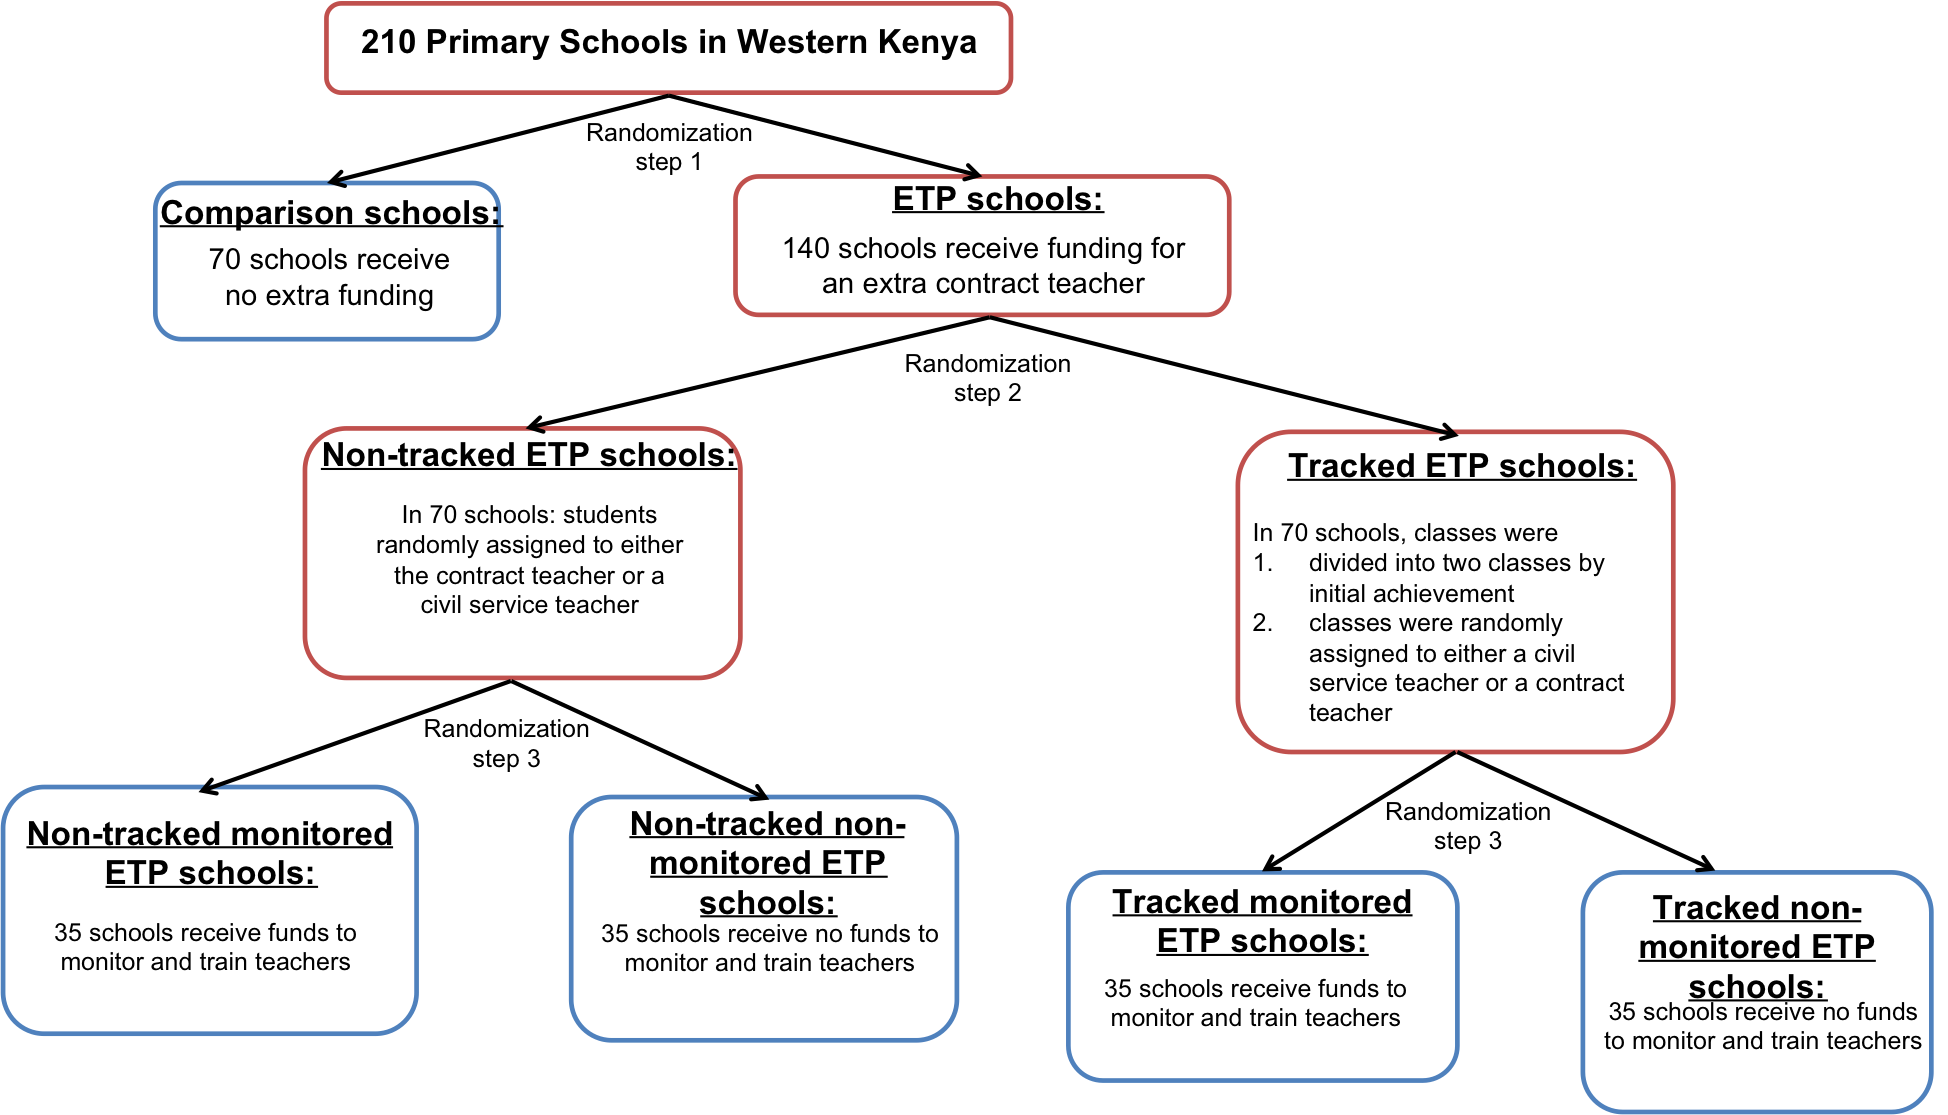
\includegraphics[scale=0.5]{Randomization_flow.png}
 \caption{A flowchart describing the randomization steps of the study}
 \label{fig:randomization}
 \end{figure}
 
Stream assignment in tracked schools was based on initial test scores (baseline test) which were administered locally within schools. Thus these baseline test scores are internally consistent within schools but not comparable across schools. The success of the program was assessed based on scores from a standardized mathematics and language test taken by 60 students from each school (approximately 7000 students all together) after 18 months (the end line test). Another test was also taken by the same students after 24 months (the long-term followup test). We note that the ETP funding ceased after the 18 month endline, so the tracking was no longer in place at the 24 month followup. These tests contained numeracy and literacy questions ranging from counting and identifying letters to subtracting two-digit numbers and writing words.
 
 \section{Exploratory Data Analysis}
 The original dataset contains observations for 7022 students over 100 variables, including individual question scores for each of the endline and follow-up tests, as well as information such as school ID, school district, whether or not the student came from a tracked or non-tracked school, gender, age, teacher-type and stream assignment (for students in the tracked schools). Although all students int he study were in the first-grade, their ages range hugely from 5 to 19, with the median age being 9 (Figure~\ref{fig:age}).
 
  \begin{figure}[h]
 \centering
 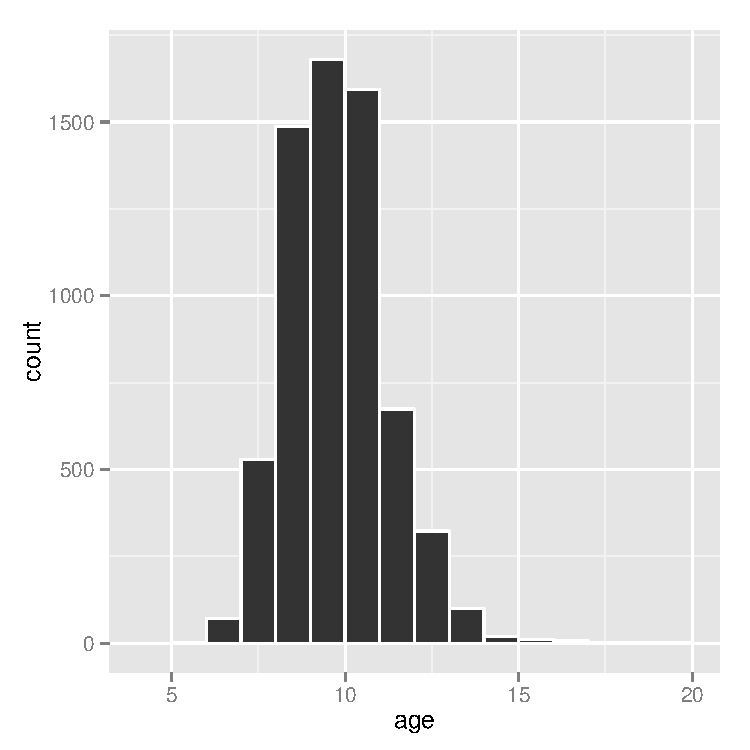
\includegraphics[scale=0.6]{age.pdf}
 \caption{Age ranges of first-grade students}
 \label{fig:age}
 \end{figure} 
 
 We compared the characteristics of students in tracking and in non-tracking schools (Table~\ref{tab:char}), and we found that in terms of age, gender and endline attrition (the percentage of students that were not present for the endline test), the students in tracked and non-tracked schools are extremely comparable. We did, however, find that the tracked and non-tracked schools are not distributed equally in terms of location. The 210 schools come from a total of 9 school zones, but we see that for Butere East and Municipality, there are approximately twice as many tracked schools as non-tracked schools, whereas for Khwisero West, there are more than twice as many non-tracked schools as there are tracked schools (Figure~\ref{fig:zone}).  Since these regions may have different education standards, we alleviate potential bias by blocking our analyses by school zone.
 
 \begin{table}[H]
 \centering
 \begin{tabular}{cccccccccc}
 \hline
 & Tracked School (n = 3613) & Non-tracked School (n = 3409)\\
 \hline
Female (\%) & 0.49 & 0.49\\
Age (mean) & 9.36 (1.47) & 9.18 (1.46)\\
Endline attrition (\%) & 0.17 & 0.17\\ \hline
 \end{tabular}
 \caption{A comparison of the characteristics of the students in tracked and non-tracked schools. The numbers in parentheses are standard deviations.}
 \label{tab:char}
 \end{table} 
 
 \begin{figure}[H]
 \centering
 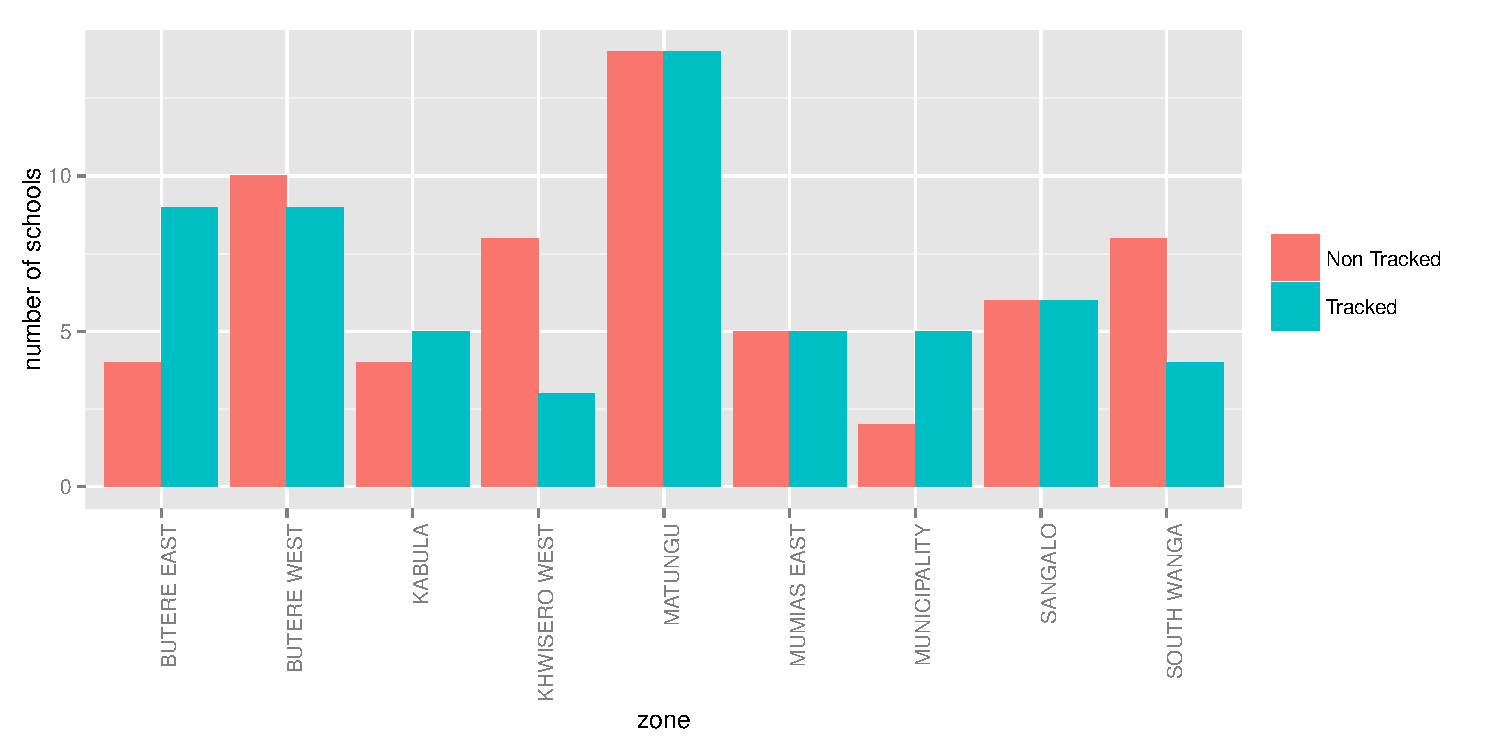
\includegraphics[scale = 0.6]{school_zones.pdf}
 \caption{The number of tracked and non-tracked schools in each school zone}
 \label{fig:zone}
 \end{figure}
 
 
 \noindent Next, for students in tracked schools, we compared the characteristics for students in the high and low stream (Table~\ref{tab:charstream}). We found that the students in the high stream were slightly older than those in the low stream and were more likely to be present at the endline test.
  \begin{table}[H]
 \centering
 \begin{tabular}{cccccccccc}
 \hline
 & Low stream (n = 1808) & High stream (n = 1805)\\
 \hline
Female (\%) & 0.49 & 0.50\\
Age (mean) & 9.14 (1.47) & 9.58 (1.44)\\
Endline attrition (\%) & 0.19 & 0.16\\ \hline
 \end{tabular}
 \caption{A comparison of the characteristics of the students in high and low streams. The numbers in parentheses are standard deviations.}
 \label{tab:charstream}
 \end{table} 
 
 
 \noindent In addition, we found concerning inconsistencies in the available data. For example the initial grade percentiles provided do not correspond to the percentiles when calculated manually (Figure~\ref{fig:percentile}). The codebook that accompanied the data stated that the provided percentiles had been imputed, although what data was used to conduct the imputation and the method of imputation is not described. We thus decided to use our own calculated percentiles for our subsequent analysis.
 
 
 \begin{figure}[H]
\centering
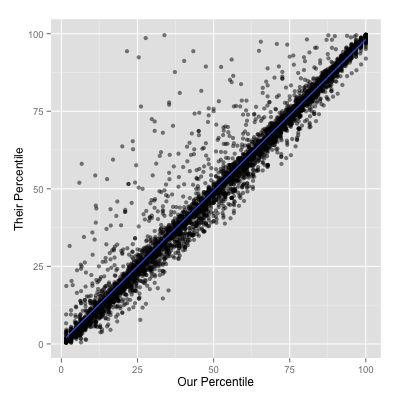
\includegraphics[scale=0.6]{Score_vs_Percentile.png}
\caption{A comparison of the percentiles reported in the data and the percentiles obtained when calculating manually.}
\label{fig:percentile}
\end{figure} 

We further note that of the 758 students without baseline scores, 756 attended non-tracking schools.  To see if the classes from the non-tracking schools mixed their high-performers and low-performers sufficiently, we compared the end-line test percentiles of each student against the average of the classmates. We found that the students' percentiles had no correlation with their peers' average percentiles, indicating that the students from the non-tracking schools whose baseline score was not provided were placed randomly into the two classes (Figure \ref{fig:NoBaselinePercentile}).

  \begin{figure}[H]
  	\centering
  	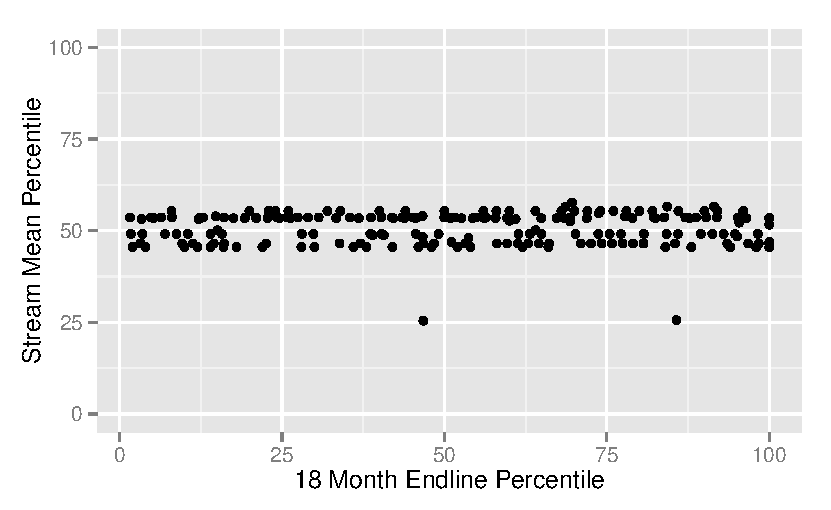
\includegraphics[scale=0.8]{../Figures/NoBaselinePercentile.pdf}
  	\caption{A comparison of endline percentiles and stream mean percentiles for all students without baseline scores.  Not having a baseline score has no correlation with classroom placement.  This turns out to be a nonissue almost all the students with no baseline score attended non-tracking schools.  The two deviate points seen in the figure belong to students in tracking schools who were placed in low streams.}
  	\label{fig:NoBaselinePercentile}
  \end{figure} 

Another issue we detected is that within tracking schools, some crossover between low and high streams occurred (Figure~\ref{fig:crossover}). We note that although this crossover is minor (only about 5.3\%), it does pose minor issues in our subsequent analyses. Duflo et al. state that the crossover was primarily due to siblings who wanted to remain in the same class, and class assignment was only changed upon a parent's request.

 
 

 
  
  \begin{figure}[ht]
 \centering
 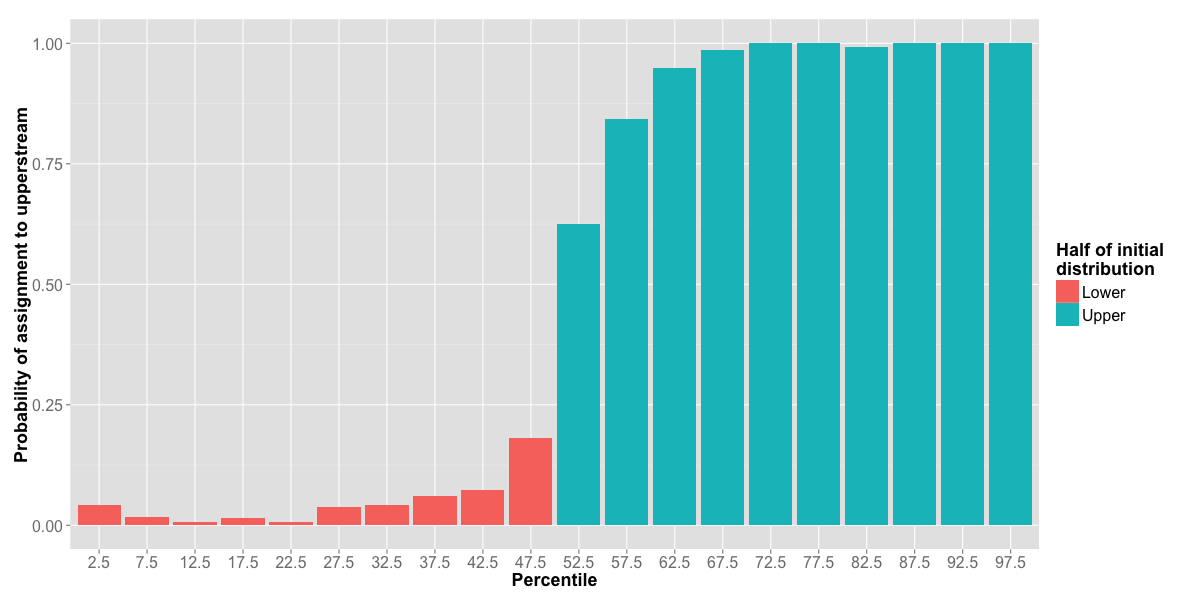
\includegraphics[scale=0.4]{tmt_assignment.png}
 \caption{The probability of assignment to high stream versus the baseline score. If no crossover occurred, the probability would be 0 until baseline score reached 0.5, after which the probability would be 1.}
 \label{fig:crossover}
 \end{figure} 
 
 
 \section{Analysis}
 \subsection{Comparing tracking with non-tracking schools at the 18 month endline}

We begin with a comparison of scores achieved by students in tracking schools with students in non-tracking schools. To perform this comparison, we tested whether tracking had an effect on the 18 month follow-up scores for students of different baseline abilities using stratified permutation tests with a t-statistic. We split students into four strata based on their percentile on their school's baseline exam score.  For this, we used the percentiles that we calculated rather than the ones supplied, due to the inconsistencies we discussed previously.  Within each stratum, we calculated the test statistic and permuted treatment assignments.  This procedure allowed us to carry out tests first within individual strata, and then for all students by taking a weighted average of the stratum-specific statistics.  Figure~\ref{fig:tracking-stratif} shows that in each stratum, tracking has a positive effect on follow-up test scores.  The effect was significant overall and for each quartile except for the third (Table~\ref{tab:tracking-stratif}, two-sided alternative). \\

  \begin{figure}[ht]
 \centering
 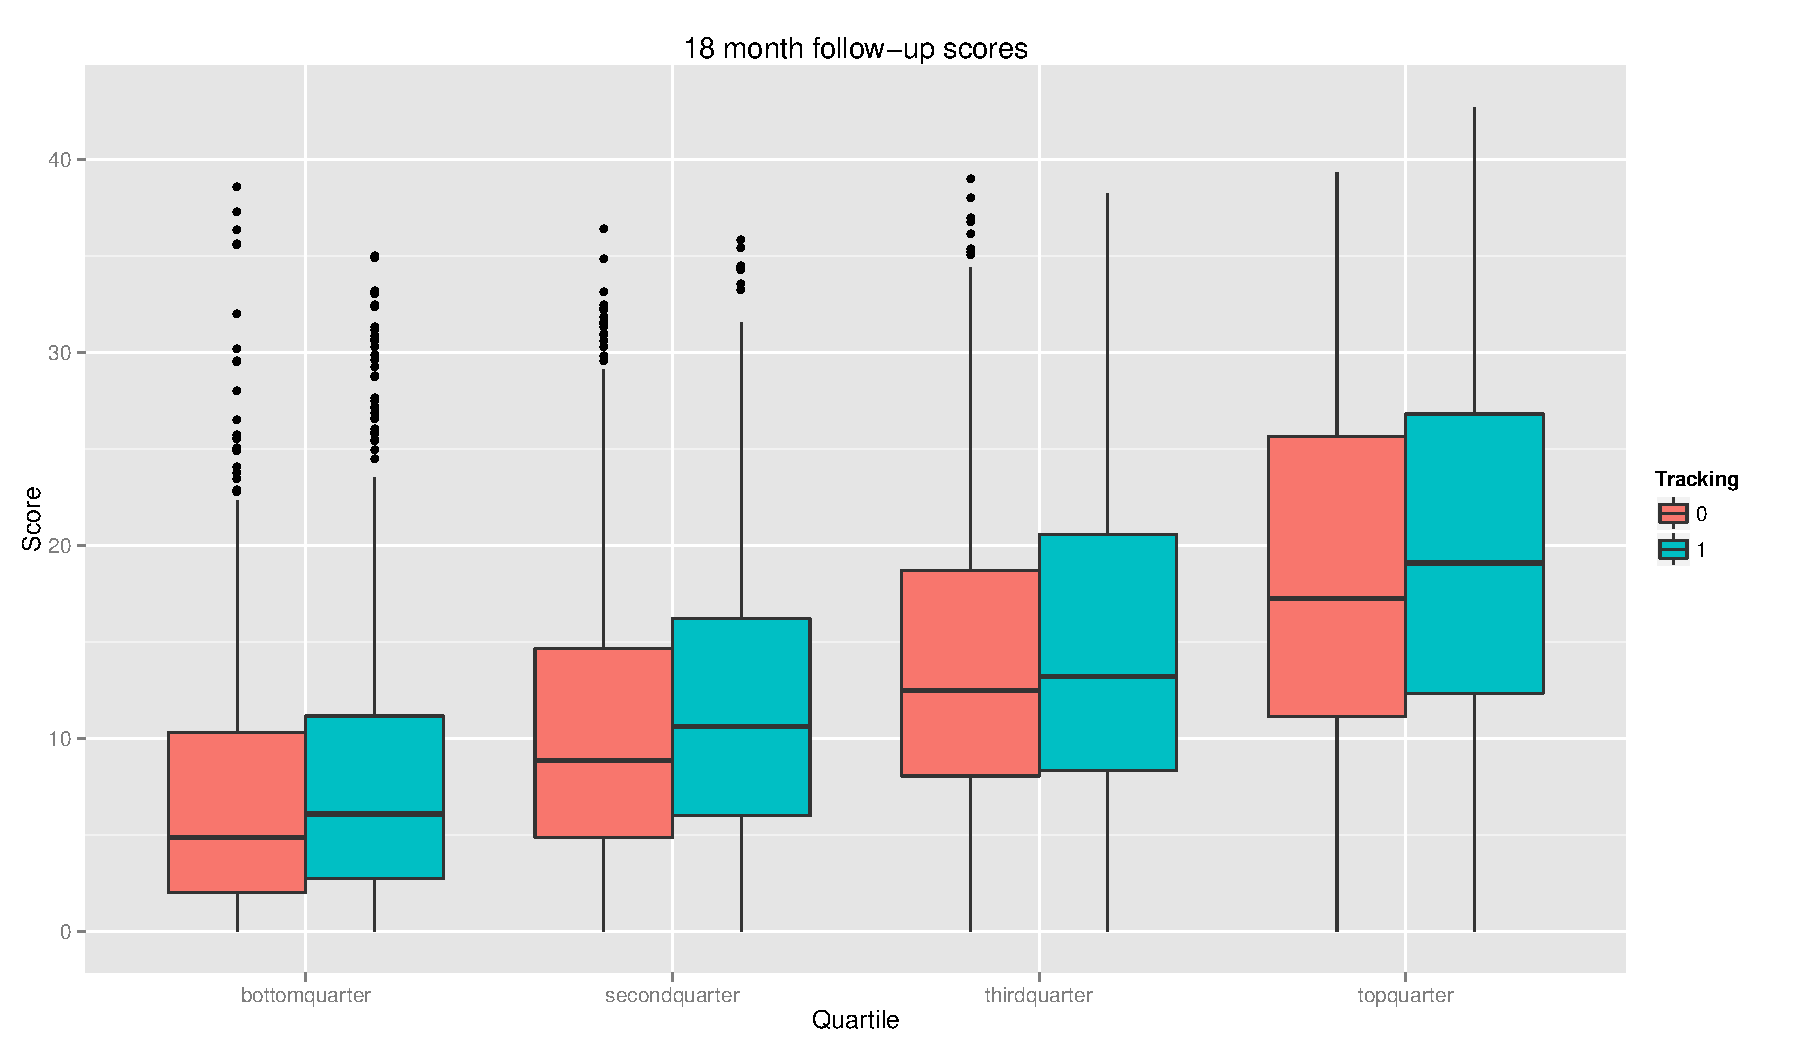
\includegraphics[scale=0.4]{tracking-stratif.pdf}
 \caption{Distribution of follow-up scores in tracking and non-tracking schools, stratified by students' quartile of baseline score}
 \label{fig:tracking-stratif}
 \end{figure} 
  % latex table generated in R 3.0.2 by xtable 1.7-4 package
% Sun Apr 26 15:37:57 2015
\begin{table}[ht]
\centering
\begin{tabular}{rrrrrr}
  \hline
 & Bottom quarter & Second quarter & Third quarter & Top quarter & Overall \\ 
  \hline
Difference in means & 0.963 & 1.318 & 0.798 & 1.425 & 1.124 \\ 
  t & 2.466 & 2.998 & 1.690 & 2.810 & 2.493 \\ 
  P-value & {\bf 0.013} & {\bf 0.003} & 0.091 & {\bf 0.005} & {\bf 0.000 }\\ 
   \hline
\end{tabular}
\caption{Test for differences in final score, stratified by baseline quartile and overall.} \label{tab:tracking-stratif}
\end{table} % Q1a in Kellie's analysis file

Next, we investigated the effect of tracking on the individual components of the 18 month follow-up score.  Table~\ref{tab:stratif-topics} shows the effect of tracking on each topic, by baseline quartile and overall.  Tracking increased students' average letter score, spelling score, literacy score, and math score.  As with the total score, the positive effects of tracking seemed to be less pronounced in the third quartile of students. \\

% latex table generated in R 3.0.2 by xtable 1.7-4 package
% Sun Apr 26 15:38:36 2015
\begin{table}[ht]
\centering
\begin{tabular}{rrrrrr}
  \hline
 & Bottom quarter & Second quarter & Third quarter & Top quarter & Overall \\ 
  \hline
Word Score & 0.048 & 0.542 & 1.017 & 1.084 & 0.661 \\ \vspace{2mm}
   & (0.963) & (0.597) & (0.319) & (0.272) & (0.188) \\ 
  Sentence Score & -0.297 & -0.761 & 0.572 & 1.173 & 0.161 \\ \vspace{2mm}
   & (0.770) & (0.450) & (0.560) & (0.235) & (0.746) \\ 
  Letter Score & {\bf 2.988} & {\bf 3.389} & {\bf 1.924} & {\bf 4.466} & {\bf 3.191} \\ \vspace{2mm}
   & {\bf (0.002)} & {\bf (0.001)} & {\bf (0.050)} & {\bf (0.000)} & {\bf (0.000)} \\ 
  Spelling Score & 1.290 & 1.111 & 0.740 & 1.689 & {\bf 1.210} \\ \vspace{2mm}
   & (0.197) & (0.268) & (0.450) & (0.093) & {\bf (0.015)} \\ 
  Literacy Score & 1.504 & 1.530 & 1.291 &{\bf  2.405} &{\bf  1.680 }\\ \vspace{2mm}
   & (0.135) & (0.131) & (0.202) & {\bf (0.015)} & {\bf (0.001) }\\ 
  Math Score & {\bf 2.869 }& {\bf 3.878} & 1.718 & {\bf 2.508 }& {\bf 2.750 }\\ 
   & {\bf (0.005)} & {\bf (0.000)} &  (0.086) & {\bf (0.011)} & {\bf (0.000) }\\ 
   \hline
\end{tabular}
\caption{t-statistics (p-values) for the test of differences in subject-level final score between tracking and non-tracking schools, stratified by baseline quartile and overall. Significant results are presented in boldface text.} \label{tab:stratif-topics}
\end{table} % Q1b in Kellie's analysis file



 \begin{figure}[H]
 \centering
 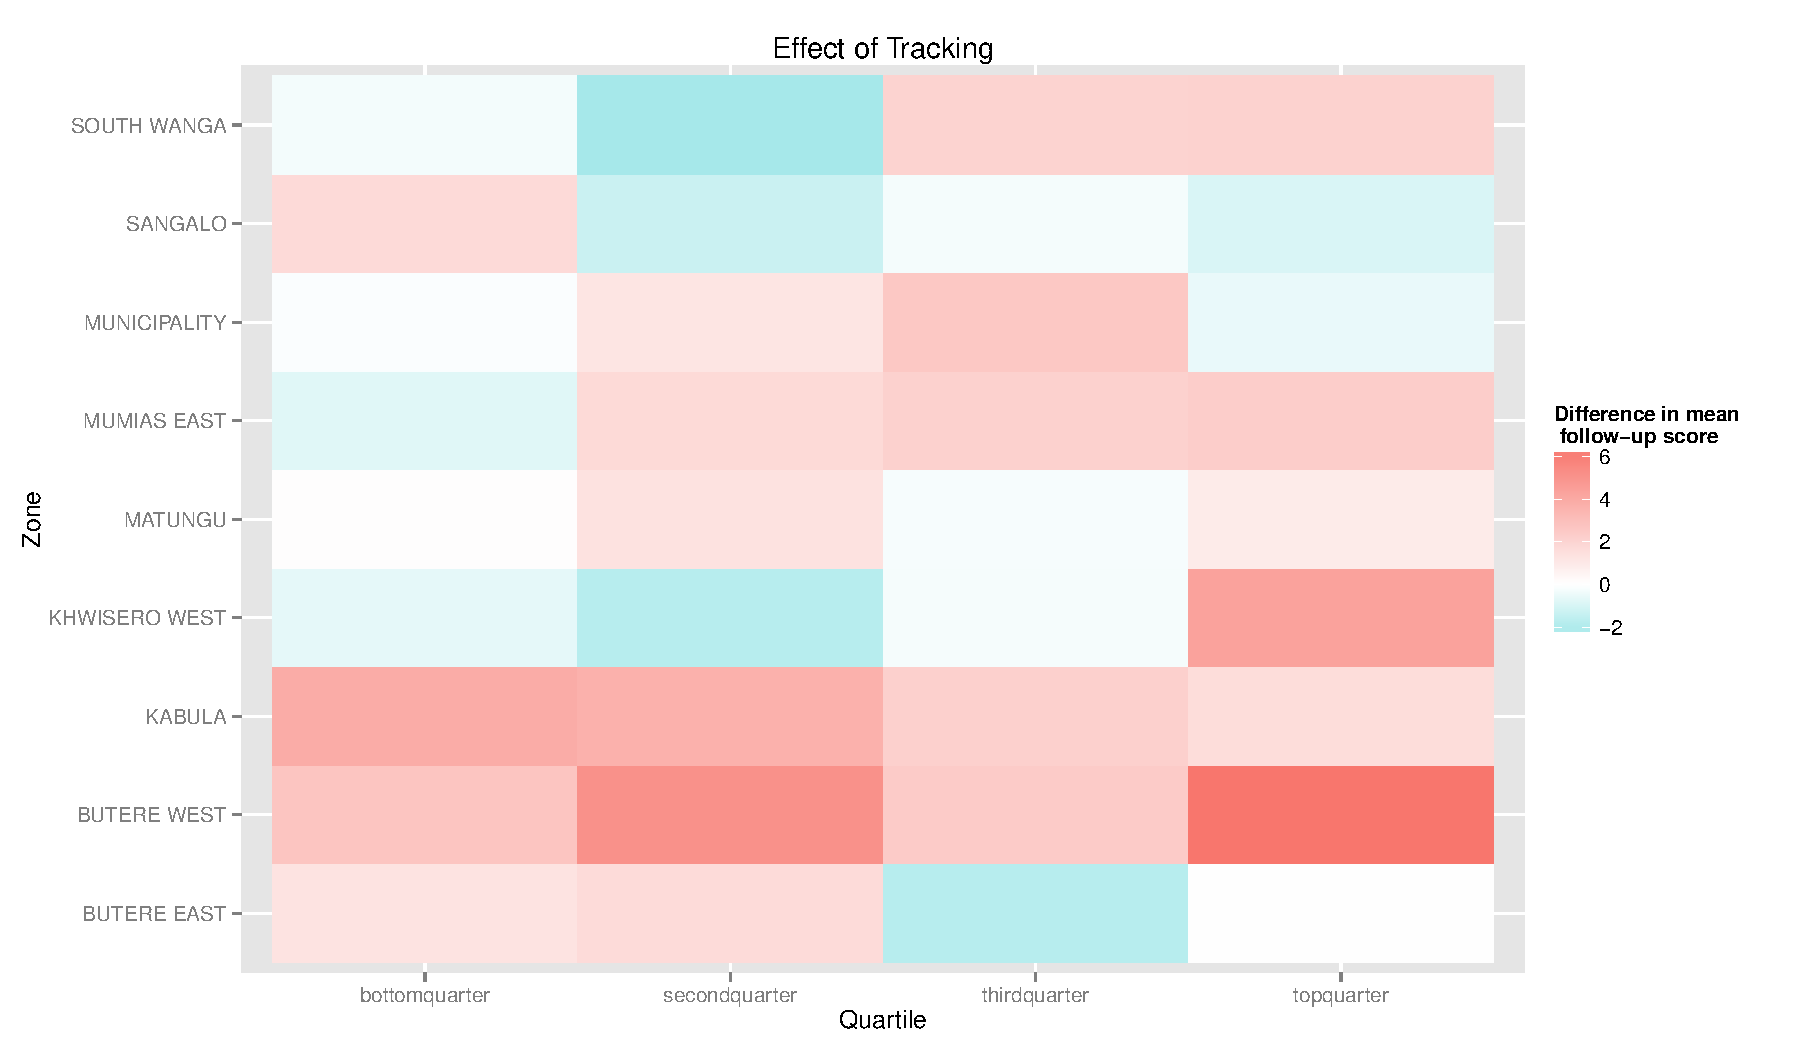
\includegraphics[scale=0.45]{tracking_by_zone.pdf}
 \caption{Difference in mean 18 month follow-up scores between students at tracking and non-tracking schools}
 \label{fig:stratif-zone}
 \end{figure}
 

We next investigated the potential bias in the estimated treatment effect due to differences in school zone.  Figure~\ref{fig:stratif-zone} shows the difference in mean 18 month follow-up scores between tracking and non-tracking schools, broken down by school zone.  The effect of tracking is heterogeneous across school zones.  While most zone-quartile combinations show a positive effect,  there are several with a negative effect in the bottom quartile.  It appears that two zones in particular, Kabula and Butere West, are driving the positive effect of tracking that we see when all zones are combined. \\

 
 \begin{figure}[h]
 \centering
 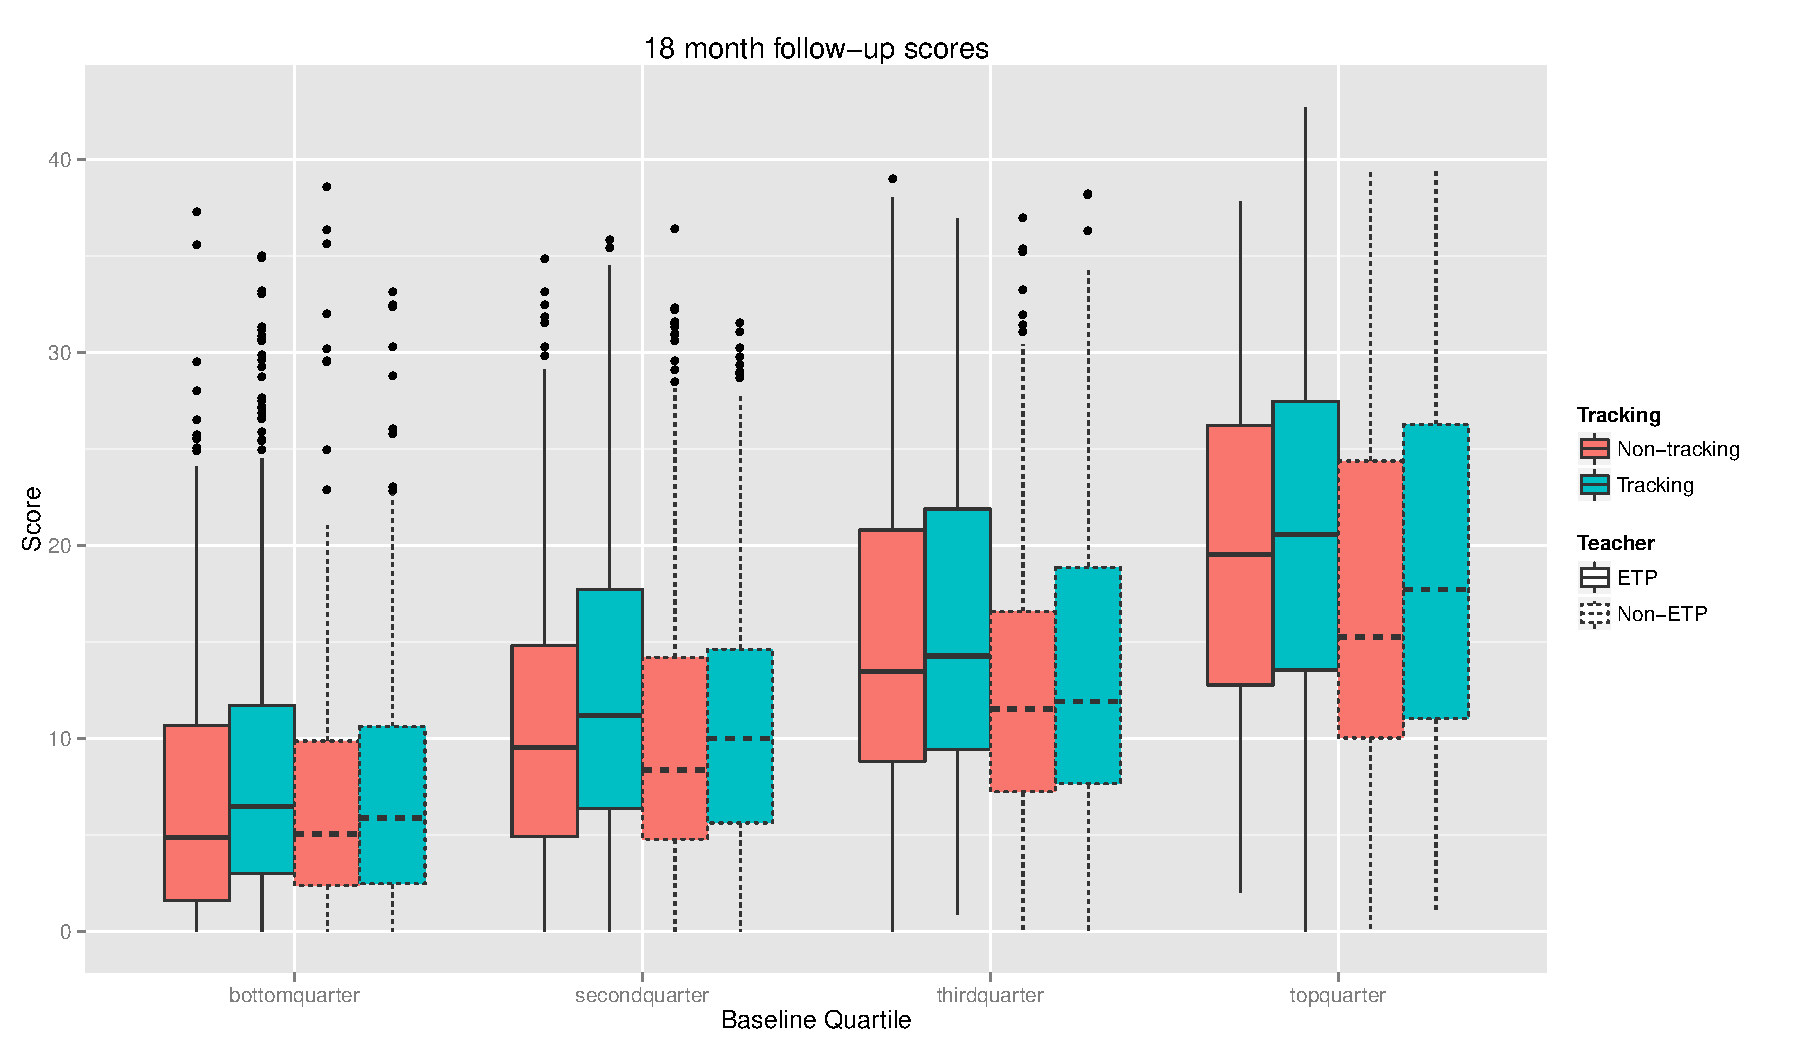
\includegraphics[scale=0.5]{tracking-etp-stratif.pdf}
 \caption{Distribution of follow-up scores in tracking and non-tracking schools, stratified by students' quartile of baseline score and type of teacher}
 \label{fig:tracking-etp}
 \end{figure}
 


Finally, we considered the possibility that the effect of tracking may be different depending on whether the teacher is a civil servant or an ETP teacher. Duflo et. al. raise the possibility that different types of teachers may teach differently; for example, ETP teachers may have a greater incentive to help the lowest quartile of students in order to secure a teaching position in the future. We did a separate stratified permutation test for each type of teacher to compare the effect of tracking on 18 month follow-up scores, for each baseline quartile and overall.  Figure~\ref{fig:tracking-etp} shows that for both types of teacher, tracking increases follow-up exam scores.  However, Table~\ref{tab:tracking-etp} presents an interesting trend.  Lower quartile students with an ETP teacher in tracking schools had a significantly higher follow-up score than those in non-tracking schools, but the effect was not as strong in the upper half of the distribution.  Conversely, students above the median with a civil service teacher had significantly higher follow-up scores in tracking schools compared to non-tracking schools, but the trend did not hold for the lower half of the distribution.  In tracking schools, the type of teacher assigned to the high and low stream has an impact on how effective tracking is.


% latex table generated in R 3.0.2 by xtable 1.7-4 package
% Sun Apr 26 18:50:55 2015
\begin{table}[ht]
\centering
\begin{tabular}{rrrrrr}
  \hline
 & Bottom quarter & Second quarter & Third quarter & Top quarter & Overall \\ 
  \hline
  ETP & {\bf 2.506} & {\bf 3.695} & 0.759 & 1.918 & {\bf 2.254 }\\ \vspace{2mm}
   & {\bf(0.011)} & {\bf (0.000) }& (0.459) & (0.061) & {\bf (0.000) }\\ 
  Non-ETP & 0.817 & 0.522 & 1.906 & {\bf 2.404 }& {\bf 1.423} \\ 
   & (0.421) & (0.611) & (0.061) & {\bf (0.017)} & {\bf (0.004)} \\ 
   \hline
\end{tabular}
\caption{t-statistics (p-values) for the test of difference in mean follow-up exam score between students in tracking vs non-tracking schools, stratified by ETP vs civil servant teachers. Significant results are presented in boldface text.}  \label{tab:tracking-etp}
\end{table} % Q5 in Kellie's analysis file

%
% \subsection{Value-added over time by tracking}
% 
%Unfortunately since the baseline test scores were not comparable across different schools, we were unable to measure the value-added from tracking by comparing baseline with the 18 month endline scores in tracking schools. As a result, we thus chose to measure the long-term value-added by comparing 18 month endline scores with the 24 month follow-up scores. This comparison allows us to see if tracking yielded a lasting effect on students, even after the tracking was no longer in place.

 \subsection{The lasting effects of tracking at the 24 month follow-up}
%Ideally the data collected would have included standardized baseline scores so we could measure the value-added from tracking by comparing baseline with the 18 month endline scores. Unfortunately, this was not how the study was designed as the baseline test scores are only consistent within schools and not across.  

We next measure the long-term value-added by comparing the 24 month follow-up scores between tracked and non-tracked schools. We can interpret this comparison as a measure of a lasting effect on students, even after the tracking was no longer in place. As seen in figure \ref{fig:va-hist}, there seems to be a remaining positive effect on the tracked students.

  \begin{figure}[H]
  	\centering
  	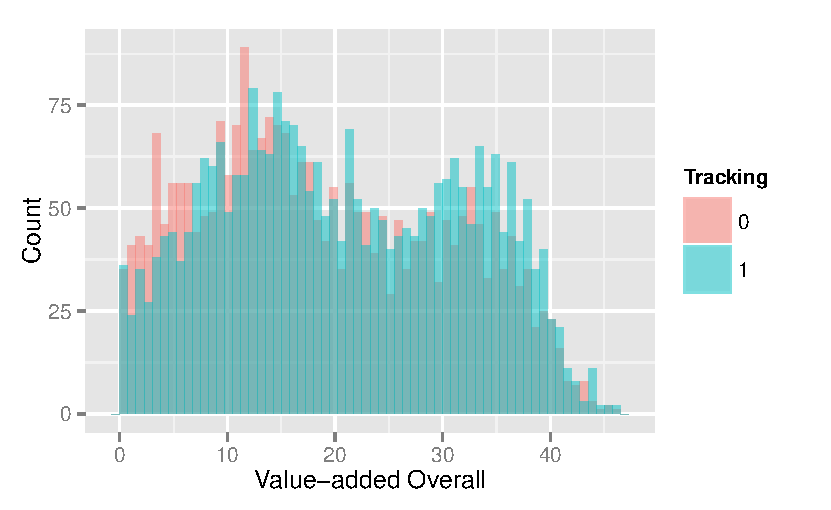
\includegraphics[scale=0.8]{../Figures/va-hist.pdf}
  	\caption{Histogram of value-added at the student level, separated by attendance at tracking and non-tracking schools.  There seems to be a slight right-shift in value-added.}
  	\label{fig:va-hist}
  \end{figure} 

We tested the significance of any observed follow-up differences between tracking and nontracking schools using permutation t-tests. To address the fact that randomization was done at the school-level, we first had to aggregate the student-level data by school, which gave us variance estimates for each of the school-level data points.  The t-statistic for the difference in means was calculated using unpooled variance and the null-distribution was approximated using 10000 random shufflings of the data within school zones (to account for the aforementioned imbalances).  The observed value-added is significant at $ \alpha = .05 $ level for all topics aside from sentence recognition and spelling. These results imply that many of the improvements yielded by tracking remain even after the tracking is no longer in place. The results of the tests can be seen in Table \ref{tab:tracking_va}.

\begin{table}[ht]
	\centering
	\begin{tabular}{rrrrrrrr}
		\hline
		& Overall & Words & Sentences & Letters & Spelling & Literacy & Math \\ 
		\hline
		Value Added & 1.600 & 1.142 & 0.859 & 3.872 & 0.391 & 0.985 & 0.611 \\ 
		t-statistic & 1.923 & 1.688 & 1.087 & 2.023 & 1.415 & 1.722 & 1.847 \\ 
		p-value & {\bf 0.030} & {\bf 0.046} & 0.143 & {\bf 0.024} & 0.081 & {\bf 0.044} & {\bf 0.035 }\\ 
		\hline
	\end{tabular}
	\caption{Test for differences between 24-month test scores} 
		\label{tab:tracking_va}
\end{table}

One could argue that the extra funding for school-based management (SBM) could be a driving force behind the increase in student performance.  However, when we tested the claim, we found no significance difference between SBM and non-SBM schools.  The results can be seen in Table \ref{tab:sbm}.  In Figure \ref{fig:ValueAddedTrackSBM}, we see that when comparing SBM-tracking to SBM-non-tracking schools, we still see a small but visible increase in the tracking schools.

\begin{table}[ht]
	\centering
	\begin{tabular}{rrrrrrrr}
		\hline
		& Overall & Words & Sentences & Letters & Spelling & Literacy & Math \\ 
		\hline
		Value Added & 1.022 & 0.559 & 0.563 & 2.709 & 0.226 & 0.600 & 0.421 \\ 
		t-statistic & 0.069 & 0.046 & 0.037 & 0.088 & 0.048 & 0.063 & 0.060 \\ 
		p-value & 0.160 & 0.400 & 0.213 & 0.124 & 0.413 & 0.236 & 0.106 \\ 
		\hline
	\end{tabular}
	\caption{Test for differences 24-month test scores in SBM and non-SBM schools.  
		Shuffling was done within school-zone groups} 
	\label{tab:sbm}
\end{table}

  \begin{figure}[H]
  	\centering
  	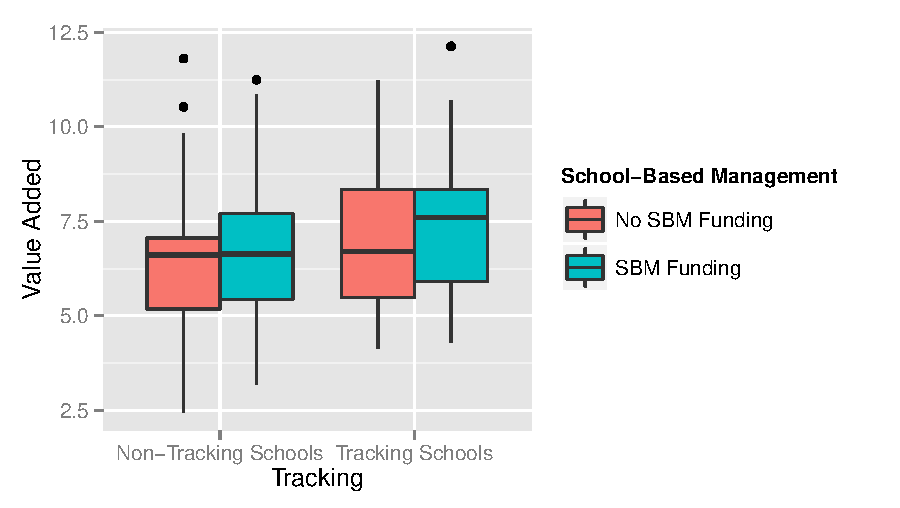
\includegraphics[scale=0.8]{../Figures/ValueAddedTrackSBM.pdf}
  	\caption{Spread of value added by tracking and participation in SBM. The small difference seen between SBM and non-SBM schools was deemed insignificant by a permutation test.  Note that even after accounting for the additional SBM funding, there is still a visible difference between tracking and non-tracking schools.}
  	\label{fig:ValueAddedTrackSBM}
  \end{figure} 

To assess the extent of improvement observed at the 24-month followup in tracked schools, we turn Table \ref{tab:practical}. The difference scores means that on average the students in tracking schools were able to identify 10\% more words, recognize 11\% more letters and be able to spell 9\% of words better than their non-tracked counterparts. Certainly the effect is not huge, but all the value-added scores are positive, suggesting that tracking, at the very least, does not have a deleterious effect in the classroom on average.


\begin{table}[ht]
	\centering
	\begin{tabular}{rrrrrrr}
		\hline
		Tracked & Word & Sent & Letter & Spelling & Math \\ 
		\hline
		 Non-tracked & 9.556 & 9.598 & 33.200 & 3.605 & 10.470 \\ 
		 Tracked & 10.536 & 10.213 & 36.947 & 3.927 & 11.079 \\ 
		\hline
		Percent increase (1dp) & 10.3 & 6.4 & 11.3 & 8.9 & 5.8\\
		\hline
	\end{tabular}
	\caption{Test for differences 24-month test scores in tracked and non-tracked schools} 
	\label{tab:practical}
\end{table}



 \subsection{The effect of stream assignment for students near the baseline cutoff}
We now aim to analyze the effect of stream assignment on students in tracked schools who initially achieved near the cutoff point. This analysis is based on the idea that students who achieved near the cutoff point have approximately equivalent abilities and it was random noise that lead to their assignment into either the high or low stream. For example, if a student slept poorly the night before the baseline test, they may have scored a few points below the cutoff point, whereas they may otherwise have scored a few points above the cutoff point. As a result, we can consider the students whose initial scores fall within a small window of the cutoff point as being randomly assigned into either the high or low stream, and we can thus evaluate the treatment effect of assignment to the high stream (for example) as if it were a random assignment for the students within some cutoff window.\\
  \begin{figure}[H]
 \centering
 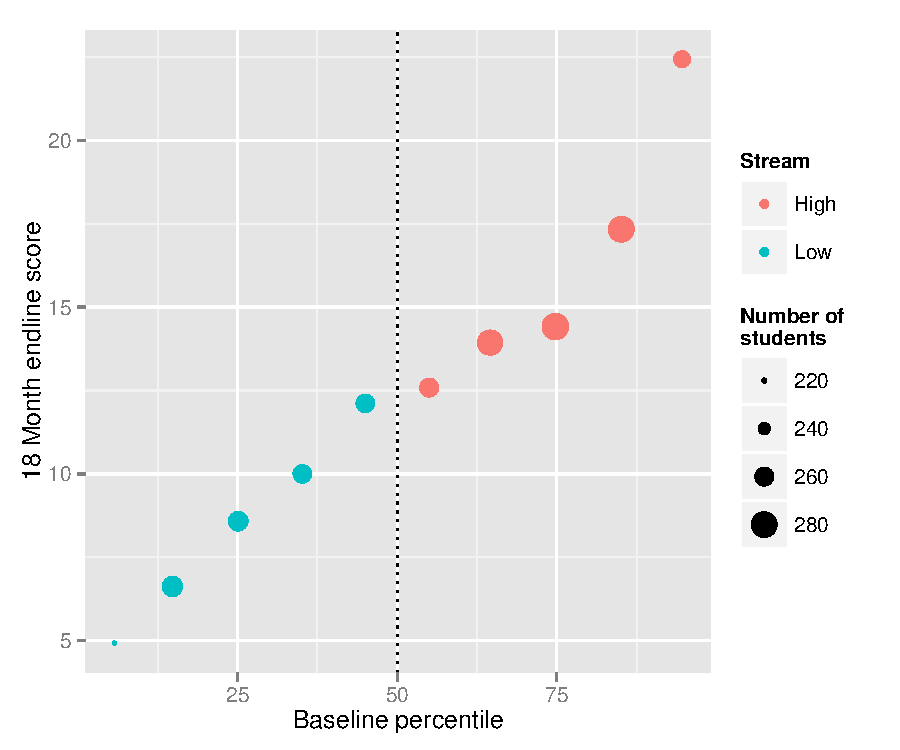
\includegraphics[scale=0.7]{RD_initial.pdf}
 \caption{Aggregated scatterplot of baseline score versus 18 month endline score. Each point is the median score of all students who fall within the corresponding score bin, each having a width of 10 percentile points. Each point is colored by the majority stream of the students in each bin.}
 \label{fig:RD_big}
 \end{figure}

When we plot the baseline score versus endline score aggregated over all students in small initial percentile bins (Figure~\ref{fig:RD_big}), visually, there does not appear to be a significant jump at the cutoff point (which is what we would expect to see in the presence of a regression discontinuity). In fact, it seems as though the slope becomes less steep, implying that assignment to the upper stream for students near the cutoff point is actually detrimental to their endline achievements.\\

 
Moreover, when zooming in on a small window around the cutoff point (Figure~\ref{fig:RD_scatter}), we see that there appears to be a discontinuity jump in the negative direction, with those students who are very close to the cutoff point but were put into the high stream appearing to perform worse than the students who were put into the low stream. Thus overall, it appears as though the students near the cutoff who are put in the low stream will perform better at the endline than those who were put in the high stream.



  \begin{figure}[ht]
 \centering
 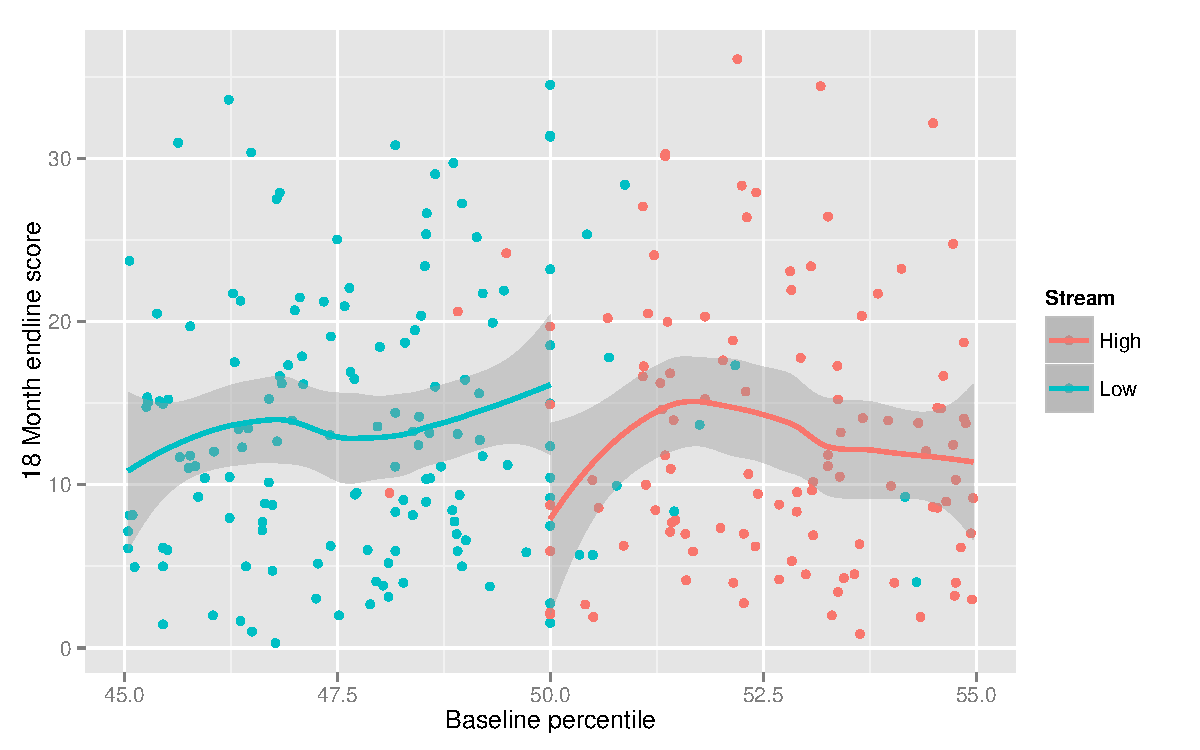
\includegraphics[scale=0.54]{RD_scatter.pdf}
 \caption{A scatterplot of baseline percentile versus 18-month score within a window of width 10 percentile points (5 percentile points in each direction around the cutoff point) with loess fitted curves for the high and low stream.}
 \label{fig:RD_scatter}
 \end{figure}
 
 Not only do we see this trend in the overall score, but when we restrict to individual subject areas, we see the same trend reflected in Literacy, Math, Spelling and Words. However, in contrast, there is a slight positive jump for Sentences and there appears to be no difference for Letters (Figure~\ref{fig:RD_scatter_subject}). \\
 




  \begin{figure}[ht]
 \centering
 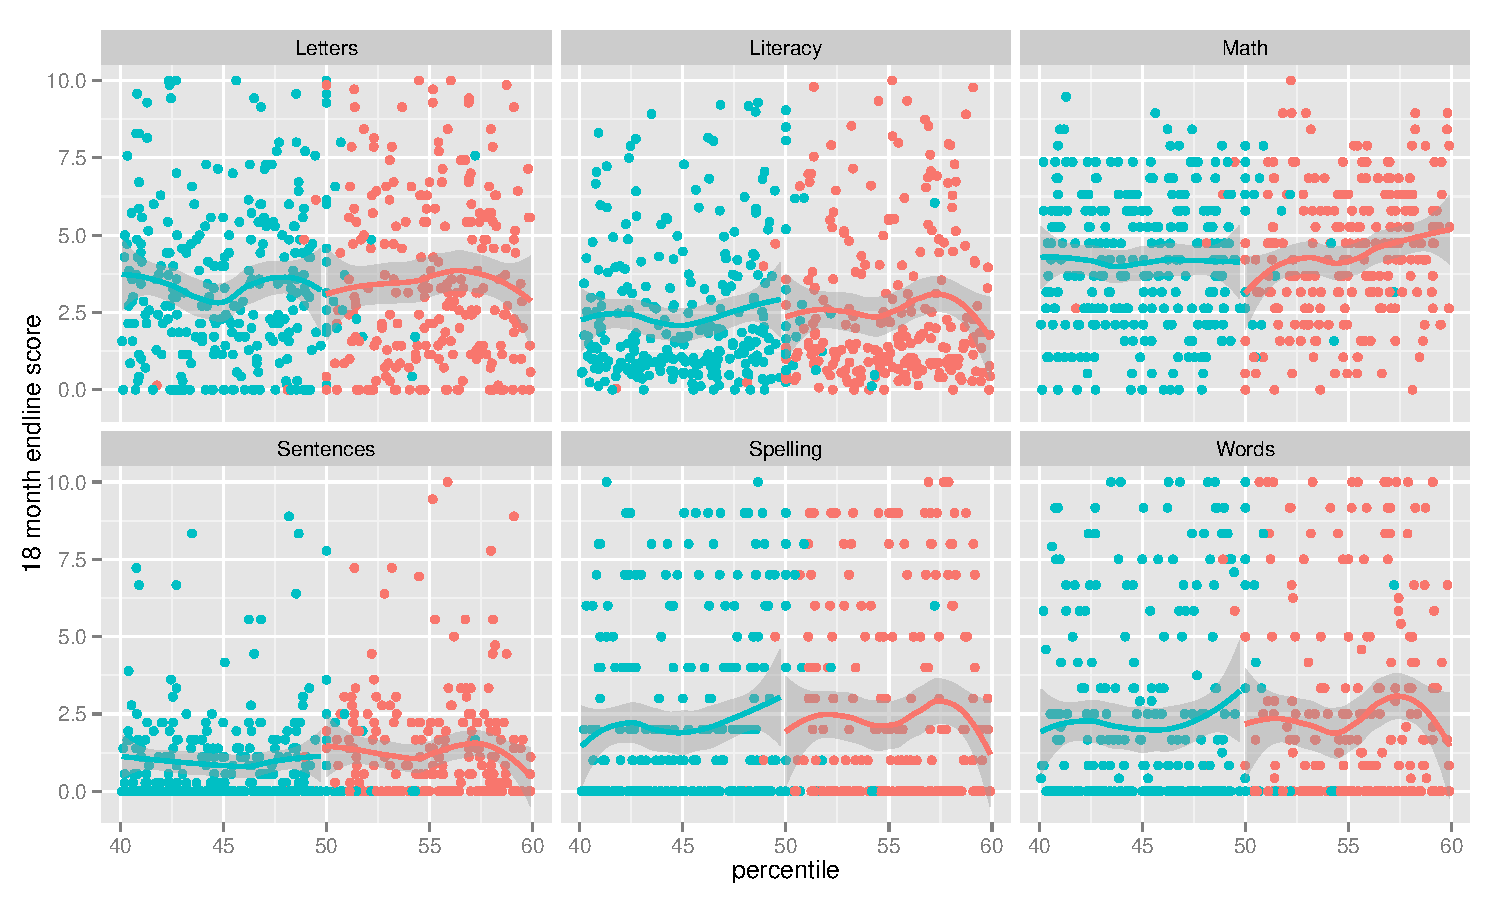
\includegraphics[scale=0.65]{RD_scatter_subject.pdf}
 \caption{Scatterplot of baseline percentile versus the standardized18-month score for each subject within a window of width 10 percentile points (5 percentile points in each direction around the cutoff point) with loess fitted curves for the high and low stream.}
 \label{fig:RD_scatter_subject}
 \end{figure}



Figure~\ref{fig:pval_window} presents the (intention to treat) $p$-values of a permutation test testing the difference in means for the overall score within each school zone, as well as the combined $p$-value from the stratified-by-zone permutation test (the rightmost cluster of bars). We see that for most school zones there is no significant difference between the students in the cutoff window who were assigned to the low stream and those who were assigned the upper stream. Further, for most school zones, the difference between high and low streams appears to increase (the p-value decreases) as we widen the window, however, we note that this is the expected result, since as we consider wider windows around the cutoff point, the difference in ability between the high and low stream students being considered increases. Thus it is surprising that for some zones, we see a decrease in difference (an increase in p-value) for example in Kabula and Matungu. The only zones for which we obtain a statistically significant difference is for the South Wanga and Sangalo school zone for the students in the 20-percentile width window about the cutoff point (the window consists of students who scored from the 40th to the 60th percentile in the baseline scores). However, this may simply be a reflection of the window being too large to still consider the students as randomly assigned to the high and low streams, and we may simply be detecting the fact that overall, the students in the high streams perform better than those in the low streams. 
 
  \begin{figure}[H]
 \centering
 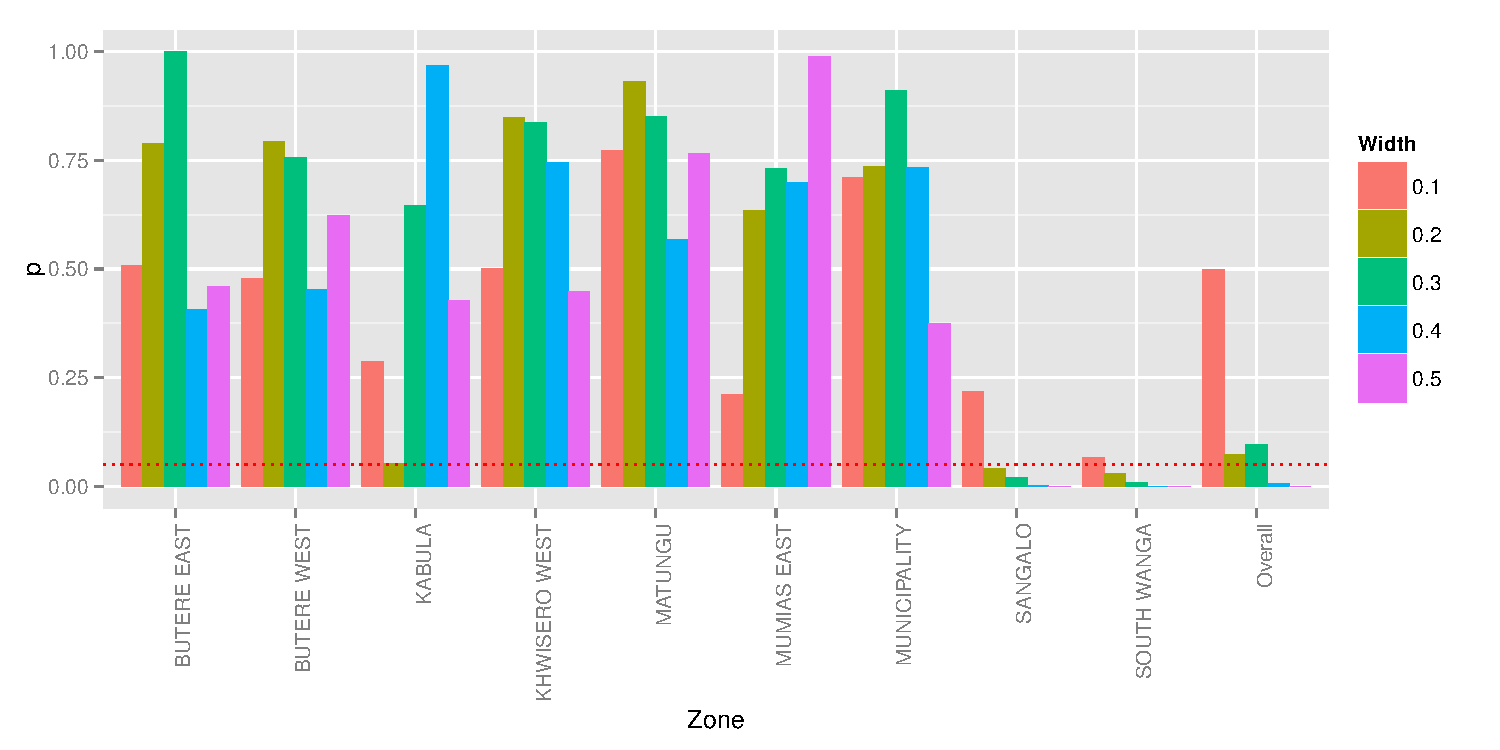
\includegraphics[scale=0.6]{RD_pval.pdf}
 \caption{Bar plot of permutation test $p$-values for differences in means between the low stream and high stream for windows of varying widths (5, 10, 15 and 20 percentile points) about the cutoff point of the 50th percentile. The 5-percentile width window contains a total of 137 students, the 10-percentile width window contains a total of 225 students, the 15-percentile width window contains a total of 405 students and the 20-percentile width window contains a total of 509 students.}
 \label{fig:pval_window}
 \end{figure}
 
 
 
 
 
 
\section{Conclusion}
We conclude that overall, tracking has a small but beneficial effect on students' learning.  After 18 months in a tracked classroom, we see that the students tend to fare better than their non-tracked counterparts in most content-areas regardless of their placement into lower and upper streams.  This positive relationship holds true for different types of teacher and for many of the school zones, although the magnitude of the effect varies. The effects of tracking seem to last even after the tracking has ceased, as we found that the differences in ability remained even six months after the program ended. We did however find that for students in tracked schools who performed near the baseline cutoff and who were assignment to the high stream did not perform as well as those assigned to the low stream. \\

Our findings are consistent with \cite{duflo2011}. Moreover, we are able to reproduce their results using non-parametric permutation tests, which make no assumptions about the distribution of noise and no assumptions about the functional relationship between tracking and exam scores. In contrast, the p-values that the authors report come from ordinary least squares regression and require normality assumptions that are difficult to check.

\bibliographystyle{apalike}
\bibliography{references}
 
\end{document}
